\apendice{Anexo de sostenibilización curricular}

\section{Introducción}
Las Naciones Unidas definen el desarrollo sostenible como aquel que satisface las necesidades del presente sin comprometer la capacidad de las generaciones futuras para satisfacer las suyas. Este principio se concreta en la \textbf{Agenda 2030 para el Desarrollo Sostenible}, adoptada en 2015, que establece \textbf{17 Objetivos de Desarrollo Sostenible (ODS)} como hoja de ruta global para erradicar la pobreza, proteger el planeta y asegurar la prosperidad para todos \cite{onuAgenda2030}.

Estos objetivos, de carácter integrador y multidimensional, afectan directamente al ámbito de la salud, la educación, la igualdad, la sostenibilidad tecnológica y el uso responsable de los recursos. El desarrollo de este Trabajo de Fin de Grado, centrado en el diseño de una herramienta digital para la predicción de trastornos del sueño mediante inteligencia artificial, se alinea con varios de estos objetivos.


\begin{figure}[H]
    \centering
    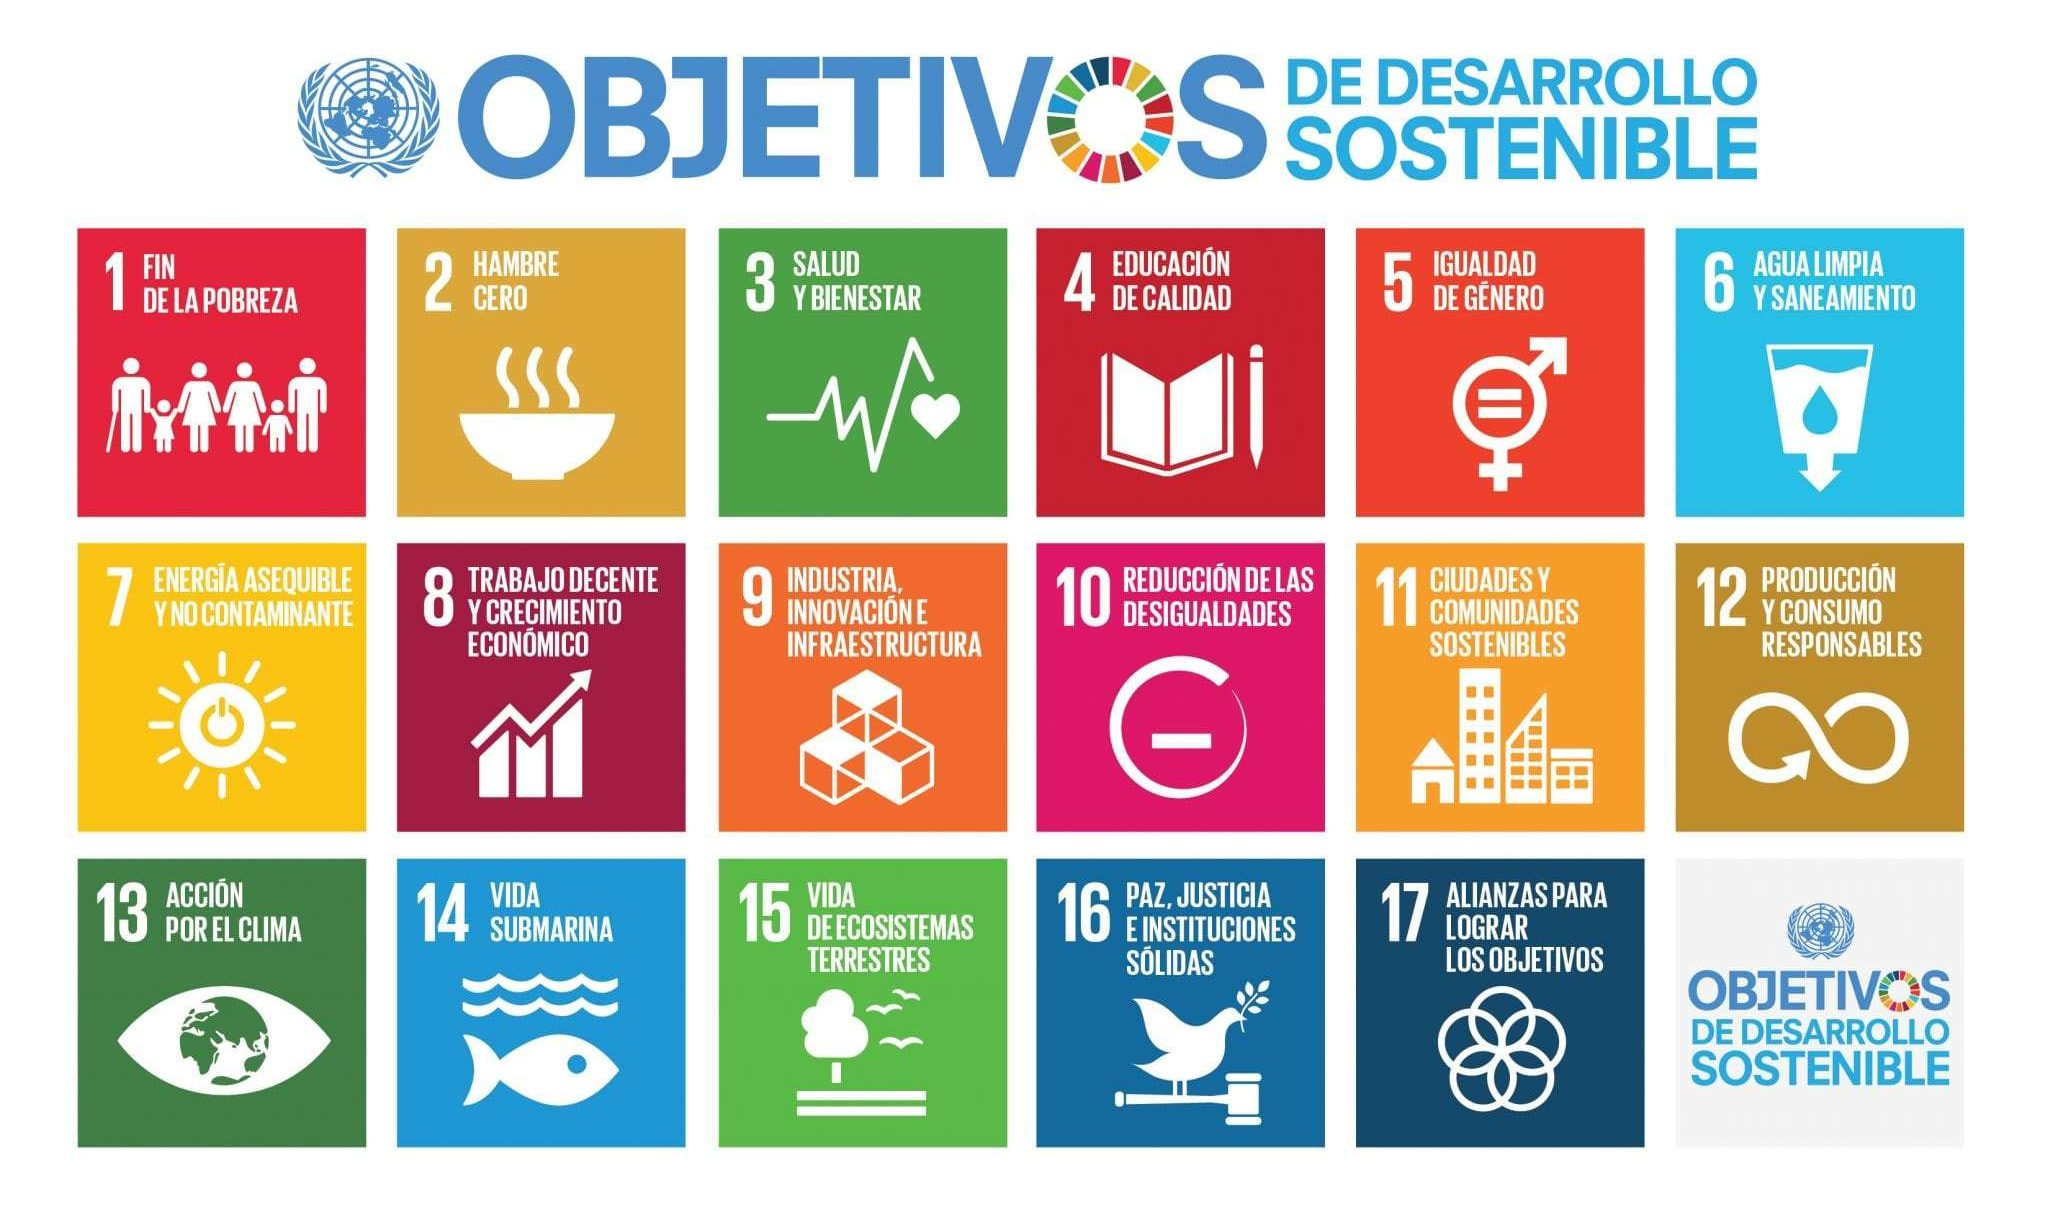
\includegraphics[width=\textwidth]{img/ODS.jpg}
    \caption{Objetivos del Desarrollo Sostenible (ODS).}
    \label{fig:ods}
\end{figure}

\subsection{ODS 3: Salud y Bienestar}

El objetivo principal del TFG ha sido el desarrollo de una herramienta predictiva de trastornos del sueño (insomnio, apnea, o sueño normal), accesible y explicable, basada en modelos de machine learning. Esta herramienta tiene un claro impacto en el ámbito del ODS 3, ya que promueve la detección temprana de problemas de salud que afectan al bienestar físico y mental de la población.

Además, el sistema facilita el acceso a la información y la concienciación sobre la importancia del sueño como parte fundamental de la salud, lo que refuerza su valor como apoyo preventivo y no invasivo. Al diseñar una interfaz intuitiva y multiplataforma, se ha buscado llegar a un público diverso, contribuyendo a mejorar el bienestar desde una perspectiva integradora y proactiva.

 
\subsection{ODS 4: Educación de calidad}
El proyecto está disponible públicamente en GitHub y documentado paso a paso para que pueda ser replicado, adaptado o ampliado por otros estudiantes o investigadores. Esta filosofía de trabajo fomenta el acceso abierto al conocimiento, promueve el aprendizaje autónomo y facilita la reutilización de recursos educativos. 

\subsection{ODS 5 y ODS 10: Igualdad de Género e Inclusión}
Desde el inicio del desarrollo del modelo predictivo se ha tenido en cuenta la importancia de evitar sesgos discriminatorios relacionados con el género u otras variables personales. El dataset empleado incluía variables como sexo, nivel de estrés, ocupación o hábitos saludables, lo que ha permitido entrenar el modelo con una perspectiva más inclusiva.

Asimismo, al tratarse de una herramienta accesible, sin barreras económicas ni tecnológicas, se contribuye a reducir las desigualdades en el acceso a recursos de salud digital, especialmente en contextos con menos recursos. El enfoque explicativo del modelo también refuerza la equidad al permitir comprender cómo influyen los factores individuales en el resultado, en lugar de presentar una predicción como una ``caja negra``.

 


\subsection{ODS 9: Industria, Innovación e Infraestructuras}
El uso de tecnologías emergentes como el aprendizaje automático, unido al desarrollo de una aplicación interactiva mediante Streamlit, representa una forma innovadora de abordar el diagnóstico preliminar en salud. La combinación entre rigor técnico y accesibilidad convierte el proyecto en un ejemplo de solución digital con vocación realista, útil y sostenible.

Además, se ha optado por el uso exclusivo de herramientas de software libre y bibliotecas mantenidas por la comunidad científica, lo que permite una implementación sin dependencia de soluciones propietarias ni altos costes de infraestructura.

 

\subsection{ODS 12: Producción y Consumo Responsables}
Durante todo el desarrollo se han priorizado prácticas sostenibles: la herramienta se ejecuta de forma digital, sin necesidad de imprimir documentación, ni utilizar recursos físicos. Tampoco requiere instalación local obligatoria, ya que está disponible en la nube, lo que reduce el impacto medioambiental y el consumo innecesario de hardware.

Del mismo modo, al evitar la generación de residuos físicos, y promover el trabajo completamente digitalizado, el proyecto encarna una forma de producción responsable basada en eficiencia, reutilización y simplicidad.


 
En conjunto, este proyecto se alinea con múltiples Objetivos de Desarrollo Sostenible al proponer una solución tecnológica accesible, educativa, ética y respetuosa con el entorno, demostrando que la innovación digital puede contribuir activamente a una sociedad más equitativa y sostenible.
